\begin{figure}[!htbp]
\vspace*{-.2cm}
\begin{center}
\tikzstyle{line} = [thick]
\tikzstyle{arw} = [->, thick,>=stealth,shorten <=2pt, shorten >=2pt]
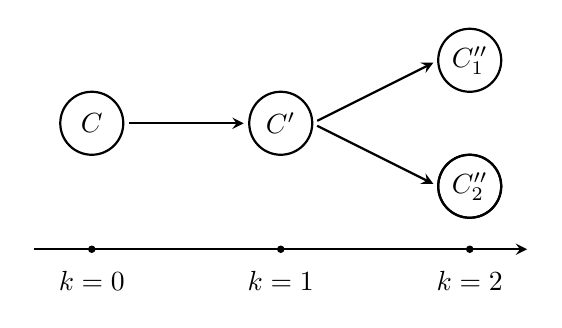
\begin{tikzpicture}

\begin{scope}[scale=0.8]
\draw [line] (-1.0,0) circle (0.5);
\draw [line] (-4.0,0) circle (0.5);
\draw [line] (2.0,1) circle (0.5);
\draw [line] (2.0,-1) circle (0.5);
\draw[arw] (-0.5,0) -- (1.5,1.0);
\draw[arw] (-0.5,0) -- (1.5,-1.0);
\draw[arw] (-3.5,0) -- (-1.5,0.0);
\node at (-4.0,0) {$C$};
\node at (-1.0,0) {$C'$};
\node at (2.0,1.0) {$C''_1$};
\node at (2.0,-1.0) {$C''_2$};
\draw [line] (2.0,-1) circle (0.5);
\draw[arw] (-5.0,-2.0) -- (3.0,-2.0);
\node at (-4.0,-2.5) {$k=0$};
\node at (-1.0,-2.5) {$k=1$};
\node at (+2.0,-2.5) {$k=2$};
\draw [fill=black] (-4.0,-2.0) circle (0.05);
\draw [fill=black] (-1.0,-2.0) circle (0.05);
\draw [fill=black] (2.0,-2.0) circle (0.05);

\end{scope}
\end{tikzpicture}
\end{center}
\vspace*{-.3cm}
\caption{Paths through an $\epsilon$-RTS}
\label{fig:krela}
\vspace*{-.3cm}
\end{figure}

\begin{figure}[!htbp]
\vspace*{-.2cm}
\begin{center}
\tikzstyle{line} = [thick]
\tikzstyle{arw} = [->, thick,>=stealth,shorten <=2pt, shorten >=2pt]
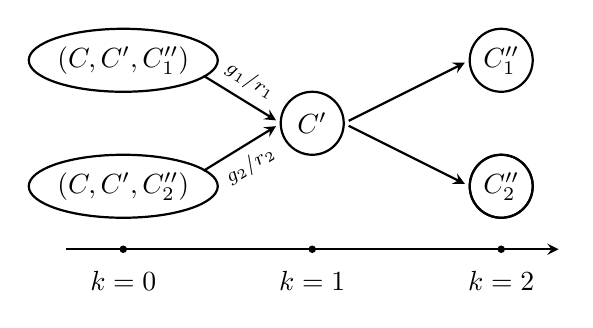
\begin{tikzpicture}

\begin{scope}[scale=0.8]
\draw [line] (-1.0,0) circle (0.5);
\draw [line] (-4.0,1) ellipse (1.5 and 0.5);
\draw [line] (-4.0,-1) ellipse (1.5 and 0.5);
\draw [line] (2.0,1) circle (0.5);
\draw [line] (2.0,-1) circle (0.5);
\draw[arw] (-0.5,0) -- (1.5,1.0);
\draw[arw] (-0.5,0) -- (1.5,-1.0);
\draw[arw] (-2.8,0.8) --
node[above,font=\fontsize{7}{7}\selectfont,sloped,pos=0.5] 
{$g_1/r_1$} (-1.5,0.0);
\draw[arw] (-2.8,-0.8) --
node[below,font=\fontsize{7}{7}\selectfont,sloped,pos=0.5] {$g_2/r_2$} (-1.5,0.0);
\node at (-4,1) {$(C,C',C''_1)$};
\node at (-4,-1) {$(C,C',C''_2)$};
\node at (-1.0,0) {$C'$};
\node at (2.0,1.0) {$C''_1$};
\node at (2.0,-1.0) {$C''_2$};
\draw [line] (2.0,-1) circle (0.5);
\draw[arw] (-5.0,-2.0) -- (3.0,-2.0);
\node at (-4.0,-2.5) {$k=0$};
\node at (-1.0,-2.5) {$k=1$};
\node at (+2.0,-2.5) {$k=2$};
\draw [fill=black] (-4.0,-2.0) circle (0.05);
\draw [fill=black] (-1.0,-2.0) circle (0.05);
\draw [fill=black] (2.0,-2.0) circle (0.05);

\end{scope}
\end{tikzpicture}
\end{center}
\vspace*{-.3cm}
\caption{Refinement of an $\epsilon$-RTS}
\label{fig:k-rel}
\vspace*{-.3cm}
\end{figure}

% We now describe how relational models can be computed for a given
% black box system by enriching the abstract reachability graph. We
% first formalize the notion of an enriched graph, and then show how
% they can be interpreted as a PWA transition system using relational
% modeling. Finally, we show how the generalization of relational
% modeling: $k$-relational modeling can be used to refine the relational
% abstraction.

% The existential abstraction relation in \cite{zutshi2014multiple} was defined as
% follows:
% \[
% %\exists \x\in\C. \exists \x'\in\C'. \x'=\simulate(\x, \tau) \iff \C\rel{\tau}\C'
%     C \areach{t} C' \iff \exists \x \in C.\ \exists \x' \in C'.\ \x \areach{t} \x'
% \]
% The abstract relation $\areach{t}$ can be enriched by incorporating
% the affine relation between $\x$ and $\x'$. For an arbitrary dynamical
% system, such a relation can be rarely represented using an exact affine map.
% This is due to the presence of non-linear and hybrid behaviors. But,
% an affine map can always be estimated with an error.
% 
% If the system dynamics are completely specified in the form of a white
% box model, we can use first order approximations to find the affine
% expressions for the relations. Using a tool like \flowstar, we can
% obtain sound over-approximate affine maps of the form $A\x + [\vb^l,
% \vb^h]$, where $[\vb^l,\vb^h]$ denotes the interval of vectors, such
% that, every element $b_i$ of the vector $\vb$ is contained in the
% respective scalar interval $b_i\in[b^l_i,b^h_i]$.
% 
% For the case of black box systems, such a sound approximation is not
% possible. Instead, we rely on statistical methods like simple linear
% regression to estimate the affine relation $f(\vx,\vx'): \x'=A\x + \vb$. We then
% estimate the error $\delta$ and generalize $\amap$ to an interval
% affine map as before $f(\vx,\vx'): \x' \in A\x + \vb + \delta$.  Finally, we get an
% abstraction with the below relation
% \[
%     C \areach{f} C' \iff \exists \x \in C.\ \exists \x' \in C'.\ \x' \in A\x + \vb \pm \delta.
%     %C \areach{A\x+\vb+\delta} C' \iff \exists \x \in C.\ \exists \x' \in C'.\
% \]
% 
% However, in the presence of complex non-linear behavior, using a
% single affine map can lead to a poor approximation. To increase the
% precision, one can use more than one affine map. Let us denote this set as
% $R_{(C,C')}$.% (ref.~\secref{ovw}).
% \[
%     R_{(C,C')}(\x,\x'): \setof{(\vx,\vx') \;|\; \exists \x \in C.\ \exists \x' \in C'.\ f(\x,\x')}
% \]
% 
% % \begin{figure}[!htbp]
% % \begin{center}
% % \tikzstyle{line} = [thick]
% % \tikzstyle{arw} = [->, thick,>=stealth,shorten <=2pt, shorten >=2pt]
% % \begin{tikzpicture}
% 
% %     \draw [line] (-1.2,-1.2) rectangle (1.2,1.2);
% %     \draw[arw] (-3,0) -- (-1.2,0);
% %     \draw[arw] (1.2,0) -- (3,0);
% 
% % \node at (-3.4,0) {$G$};
% % \node at (3.4,0) {$G^R$};
% % \node[align=center] at (0, 0) {\scriptsize Enrich using \\ \scriptsize Regression \\ \scriptsize(OLS)};
% 
% % \end{tikzpicture}
% % \end{center}
% % \vspace*{-.3cm}
% % \caption{Using OLS, $G^R$ is computed by determining the appropriate
% % $R_{(C,C')}$ for each edge of $G$.}
% % \label{fig:enrichment}
% % \vspace*{-.3cm}
% % \end{figure}
% 
% As shown in \figref{enrichment}, we use OLS to compute an enrichment
% of the abstraction graph $G$. For every edge $(C,C') \in edges(G)$,
% the set of relations $R_{(C,C')}(\x,\x')$ is computed. The semantics
% of the enriched edge are non-deterministic. Form a state $\x
% \in C$, any $f\in R_{(C,C')}$ can be taken as long as $\x' \in C$'
% is satisfied. This interpretation results in an infinite state
% transition system. We now detail the construction of the set
% $R_{(C,C')}$ using $k$-relational modeling.
% 
% % We now compute a PWA model for a given black box system by estimating
% % the dynamics using OLS. We can estimate the affine relations between
% % every cell, but as discussed in ~\chapref{abs}, it is a futile
% % approach.  Instead, we use the same heuristic as before:
% % scatter-and-simulate, to select the cell relations for estimation. We
% % build the reachability graph as before, but in addition, annotate each
% % edge with the values of estimated $A$, $\vb$, and $\delta$ for the
% % respective relation. The reachability graph thus computed, is a
% % transition system. Using off-the-shelf bounded model checkers, we
% % reason about the system's safety properties.

In this section, we show a technique to refine an $\epsilon$-RTS that
does not incur the curse of dimensionality faced by the CEGAR-based
refinement procedure for $\epsilon$-TS abstractions. The main idea is
still to split cells of the $\epsilon$-RTS; however, cells are not
split spatially.  Instead, we re-define a cell as a tuple, the first
element of which is the original cell number (indicating the
equivalence class generated by the quantization function), and the
subsequent $k$ elements indicate the indices of the $k$ cells through
which a trajectory originating in the cell may pass. We call such a
representation a $k$-relational $\epsilon$-RTS, or $(k,\epsilon)$-RTS
for short. 

To further, explain, let us consider a $2$-relational $\epsilon$-RTS.
Consider Figure~\ref{fig:krela}. The intuitive idea for the
$k$-relational $\epsilon$-RTS abstraction is that a trajectories that
follow the path $C \rightarrow C' \rightarrow C_1''$ typically obey a
{\em different} guard/update relation going from cell $C$ to $C'$ than
trajectories following the path $C \rightarrow C' \rightarrow C_2''$.
Thus, based on the cell of eventual destination, we can split the cell
$C$ into two cells: $(C,C',C_1'')$ and $(C,C',C_2'')$. Furthermore, we
can identify different guard/update relation on the transition from
these cells to cells of the form $(C',*,*)$ as shown in
Figure~\ref{fig:krelb}. Here $*$ denotes any arbitrary cell. In other
words the ``trajectory bundle'' corresponding to simulations from cell
$C$ to $C'$ now is split into two bundles, based on where the
trajectories from each bundle may end up in two steps.

Suppose we are given an $\epsilon$-RTS
$(\Cells,\vx,\CellEdges,\InitCells,\CellLabelingFunction,\EdgeLabelingFunction,\UnsafeStates)$,
then, a $(k,\epsilon)$ is defined as a tuple: $(\kCells, \vx,
\kCellEdges, \kInitCells, \kCellLabelingFunction,
\kEdgeLabelingFunction)$, where:

\begin{itemize}[label=--,leftmargin=1em,labelsep=*]
\item
$\kCells \subset \Cells^k$, \\
\item
$\kCellEdges \subset \kCells \times \kCells$, \\
\item
$(C_1,\ldots,C_k) \in \kInitCells$ iff $C_1 \in \InitCells$, \\
\item
$\kCellLabelingFunction((C_1,\ldots,C_k))$ =
$\CellLabelingFunction(C_1)$, \\
\item
$\kEdgeLabelingFunction((C_1,\ldots,C_k),(C'_1,\ldots,C'_k)) =
(g(\vx),r(\vx,\vxp))$, as before.
\end{itemize}

The operational semantics of a $(k,\epsilon)$-RTS are similar to that
of an $\epsilon$-RTS. The key difference is in how it is constructed.
We note that the $\epsilon$-RTS introduced in Sec.~\ref{sec:scamr} is
basically a $1$-relational $\epsilon$-RTS.


% 
% Given $G$, when computing the set of relations $R$ for an edge, we
% consider only the set of abstract states reachable at a specific time
% step.  Intuitively, one might consider the states reachable in one
% time step $\Delta$.  However, such a process can be generalized by
% looking at the states reachable at ${0\Delta, 1\Delta, \ldots,
% k\Delta}$ time steps. We denote these states as $\vx, \vx', \ldots
% \vx^k$.

% Using \figref{k-rel}, we illustrate this notion. To compute
% $R_{(C,C')}$, we
% split the data set $\ds(C,C')$ consisting of trajectory segments of time lengths
% $k\Delta$ as follows.  We observe the local behavior of the system by
% noting the evolution of the system $\System$ from a state $\vx \in C$
% reachable at time $t$ for a time length dependant on $k$. For
% \begin{itemize}
%     \item{$k=0$}: we observe all trajectory segments of length $\Delta$.
%     \item{$k=1$}: we observe trajectory segments of length $\Delta$,
%         which satisfy $\vx'\in C'$, where $\vx'$ is reachable from
%         $\vx$ in time $\Delta$.
%     \item{$k=2$}: we observe trajectory segments of length $2\Delta$,
%         and split them in two sets (a) and (b) on the basis of the
%         cells reached at time $(t+\Delta)$ and $(t+2\Delta)$.
%         \begin{enumerate}[label=\alph*]
%             \item $\x' \in C' \land \x''\in C''_1$
%             \item $\x' \in C' \land \x'' \in C''_2$
%         \end{enumerate}
%     \item{$k=n$}: we observe trajectory segments of length $n\Delta$,
%         and split them in to multiple sets on the basis of the cells
%         reached at time $(t+\Delta),\; (t+2\Delta),\;
%         \ldots,\;(t+n\Delta)$.
% \end{itemize}
% 
% $k$-relational modeling can be understood as a heuristic, which uses
% the underlying abstraction to differentiate behaviors of the system
% which `diverge' (or are revealed to be `distinct' at a future time).
% Such a heuristic can be useful in increasing the precision of the
% learnt affine maps.  We now formalize this notion for $k=0$, $1$, and
% $n$ and illustrate using examples.

% \mypara{$0$-Relational Model}
% 
% \begin{figure}[!htbp]
% \begin{center}
% \tikzstyle{line} = [thick]
% \tikzstyle{arw} = [->, thick,>=stealth,shorten <=2pt, shorten >=2pt]
% \begin{tikzpicture}
% \begin{scope}[scale=0.8]
% 
%     \draw [line] (-1.0,-1.0) rectangle (1.0,1.0);
%     %\draw [line] (3.0,1.0) rectangle (5.0,3.0);
%     %\draw [line] (3.0,-3.0) rectangle (5.0,-1.0);
%     \draw [line] (-0.7,0.5) .. controls +(2.0,2.0) and +(-2.0,-2.0) ..  (3.5,2.2);
%     \draw [line] (-0.5,0.0) .. controls +(2.0,2.0) and +(-2.0,-2.0) ..  (3.5,1.7);
%     \draw [line] (-0.0,-0.5) .. controls +(2.0,2.0) and +(-2.0,-1.0) ..  (3.5,-1.2);
% 
% \node at (0.0, 0.0) {$C$};
% \node at (-0.75,0.7) {\scriptsize{$\x_0$}};
% \node at (3.7,2.2) {\scriptsize{$\x_0'$}};
% \node at (-0.7,0.0) {\scriptsize{$\x_1$}};
% \node at (3.7,1.7) {\scriptsize{$\x_1'$}};
% \node at (-0.2,-0.5) {\scriptsize{$\x_2$}};
% \node at (3.7,-1.2) {\scriptsize{$\x_2'$}};
% \node at (2,1.5) {$\pi_1$};
% \node at (2,0.5) {$\pi_2$};
% \node at (1.7,-1) {$\pi_3$};
% \draw[arw] (-1.5,-2.0) -- (4.5,-2.0);
% \node at (0,-2.5) {$t=0$};
% \node at (4,-2.5) {$t=\Delta$};
% \draw [fill=black] (0.0,-2.0) circle (0.05);
% \draw [fill=black] (4.0,-2.0) circle (0.05);
% 
% \end{scope}
% \begin{scope}[xshift=0,yshift=2.1cm,scale=0.5]
%     \node at (2,0) {\footnotesize $\scr{T} \equiv g_1(\x):\vx \in C
%     \implies \vx' \in A_1\vx + \vb_1 + \delta_1$};
% \end{scope}
% 
% \end{tikzpicture}
% \end{center}
% \vspace*{-.3cm}
% \caption{All the trajectory segments will be used to construct the
% model; $\ds = \setof{\pi_1, \pi_2, \pi_3}$.}
% \label{fig:k0}
% \vspace*{-.3cm}
% \end{figure}
% 
% When $k=0$, the $0$-relational model is a PWA transition system which only
% defines the evolution of states $\x$, and does not specify the
% reachable cell. The guard predicates of the relations are defined over
% cells: $g_i(\x): \x \in C_i$ while $g'_i(\x'): True$.
% 
% We use regression to estimate the dynamics for the outgoing trajectory
% segments form a cell $C$. Hence, the data set $\ds$ for the regression
% includes all trajectory segments beginning from the same cell
% \[
%     \ds = \setof{(\vx,\vx') | \vx \in C}.
% \]
% This includes trajectory segments ending in different cells, as shown
% in ~\figref{k0}. For $N$ cells, this results in a $\rho$ with $N$ transition relations.
% \begin{equation*}
%     \scr{T} = \left\{
%         \begin{array}{ll}
%             g_1(\x):\vx \in C_1 \implies \vx' \in A_1\vx + \vb_1 + \delta_1\\
%             \ldots \\
%             g_n(\x):\vx \in C_n \implies \vx' \in A_n\vx + \vb_n + \delta_n\\
%         \end{array}
%     \right.
% \end{equation*}
% 
% Note that this can be quite imprecise when the cells are big,
% containing regions of state-space with complex dynamics. This is true
% for both non-linear systems and hybrid dynamical system, where a cell
% can contain two or more modes with differing continuous dynamics.
% 
% \mypara{$1$-Relational Model}
% 
% \begin{figure}[!htbp]
% \begin{center}
% \tikzstyle{line} = [thick]
% \tikzstyle{arw} = [->, thick,>=stealth,shorten <=2pt, shorten >=2pt]
% \begin{tikzpicture}
% \begin{scope}[scale=0.8]
% 
%     \draw [line] (-1.0,-1.0) rectangle (1.0,1.0);
%     \draw [line] (3.0,1.0) rectangle (5.0,3.0);
%     \draw [line] (3.0,-3.0) rectangle (5.0,-1.0);
%     \draw [line] (-0.7,0.5) .. controls +(2.0,2.0) and +(-2.0,-2.0) ..  (3.5,2.2);
%     \draw [line] (-0.5,0.0) .. controls +(2.0,2.0) and +(-2.0,-2.0) ..  (3.5,1.7);
%     \draw [line] (-0.0,-0.5) .. controls +(2.0,2.0) and +(-2.0,-1.0) ..  (3.5,-1.2);
% 
% \node at (0.0, 0.0) {$C$};
% \node at (4.0, 2.0) {$C'_1$};
% \node at (4.0, -2.0) {$C'_2$};
% \node at (-0.75,0.7) {\scriptsize{$\x_0$}};
% \node at (-0.7,0.0) {\scriptsize{$\x_1$}};
% \node at (-0.2,-0.5) {\scriptsize{$\x_2$}};
% \node at (3.3,2.5) {\scriptsize{$\x_0'$}};
% \node at (3.7,1.5) {\scriptsize{$\x_1'$}};
% \node at (3.7,-1.5) {\scriptsize{$\x_2'$}};
% \node at (2,1.5) {$\pi_1$};
% \node at (2,0.5) {$\pi_2$};
% \node at (1.7,-1) {$\pi_3$};
% \draw[arw] (-1.5,-3.5) -- (5.5,-3.5);
% \node at (0,-4.0) {$t=0$};
% \node at (4,-4.0) {$t=\Delta$};
% \draw [fill=black] (0.0,-3.5) circle (0.05);
% \draw [fill=black] (4.0,-3.5) circle (0.05);
% 
% \end{scope}
% \begin{scope}[xshift=1cm,yshift=3.1cm,scale=0.5]
%     \node at (2,0) {\begin{minipage}{\linewidth}
%     \footnotesize \begin{equation*}
%         \scr{T} = \left\{
%         \begin{array}{ll}
%             g_1(\x):\vx \in C \land g'_1(\x):\vx \in C'_1 \implies \vx' \in A_1\vx + \vb_1 + \delta_1\\
%             g_2(\x):\vx \in C \land g'_2(\x):\vx \in C'_2 \implies \vx' \in A_2\vx + \vb_2 + \delta_2
%         \end{array}
%     \right.
% \end{equation*}
% \end{minipage}};
% \end{scope}
% 
% \end{tikzpicture}
% \end{center}
% \vspace*{-.3cm}
% \caption{The data gets split into two sets $\ds_1 = \setof{\pi_1,
%     \pi_2}$ and $\ds_2 = \setof{\pi_3}$ and two relations:
%     $R_{(C,C'_1)}$ and $R_{(C,C'_2)}$, each with one affine map, are constructed.}
% %Cardinality($R_{(C,C')}$) = $2$.}
% \label{fig:k1}
% \vspace*{-.3cm}
% \end{figure}
% 
% 
% % \begin{scope}[xshift=0,yshift=4.0cm,scale=1]
% %     \node at (2,0) {\footnotesize $\begin{equation*}
% %     \scr{T} = \left\{
% %         \begin{array}{ll}
% %             g_1(\x):\vx \in C \land g'_1(\x):\vx \in C'_1 \implies A_1\vx + \vb_1 + \delta_1\\
% %             g_2(\x):\vx \in C \land g'_2(\x):\vx \in C'_2 \implies A_2\vx + \vb_2 + \delta_2
% %         \end{array}
% %     \right.
% % \end{equation*}$};
% % \end{scope}
% 
% To improve the preciseness of learnt dynamics, we include the
% reachability relation in the
% regression. For every relation $C\areach{t}C'$, the data set $\ds$ is
% comprised only of trajectory segments $\pi_t$ which start and end in
% the same set of cells.
% \[
%     \ds = \setof{(\vx,\vx') | \vx \in C \land \vx' \in C'}.
% \]
% For $N$ edges in $G$, $1$-relationalization results in a $\rho$ with
% $N$ transition relations.  \figref{k1} illustrates the $k=1$ refinement of the case shown in
% \figref{k0}. The data set $\ds$ is split into two data sets $\ds_1
% = \setof{\pi_1, \pi_2}$ and $\ds_2 = \setof{\pi_3}$, using which, two
% relations are constructed. The resulting $1$-relational model
% is at least as precise as the corresponding $0$-relational model.

\mypara{$k$-Relational Model}

\begin{figure}[!htbp]
\begin{center}
\tikzstyle{line} = [thick]
\tikzstyle{arw} = [->, thick,>=stealth,shorten <=2pt, shorten >=2pt]
\begin{tikzpicture}
\begin{scope}[xshift=0cm, scale=0.75]

    \draw [line] (-1.0,-1.0) rectangle (1.0,1.0);
    \draw [line] (3.0,1.0) rectangle (5.0,3.0);
    %\draw [line] (3.0,-3.0) rectangle (5.0,-1.0);
    \draw [line] (7.0,1.0) rectangle (9.0,3.0);
    \draw [line] (7.0,-3.0) rectangle (9.0,-1.0);
    \draw [line] (-0.7,0.5) .. controls +(2.0,2.0) and +(-2.0,-2.0) .. (3.5,2.2) .. controls +(2.0,2.0) and +(-2.0,-2.0) .. (8.5,1.8) ;
    \draw [line] (-0.5,0.0) .. controls +(2.0,2.0) and +(-2.0,-2.0) .. (3.5,1.7) .. controls +(2.0,2.0) and +(-2.0,-2.0) .. (8.5,-2.2) ;

%     \draw [line] (-0.7,0.5) .. controls +(2.0,2.0) and +(-2.0,-2.0) ..  (3.5,2.2);
%     \draw [line] (-0.5,0.0) .. controls +(2.0,2.0) and +(-2.0,-2.0) ..  (3.5,1.7);

    %\draw [line] (-0.0,-0.5) .. controls +(2.0,2.0) and +(-2.0,-1.0) ..  (3.5,-1.2);

\node at (0.0, 0.0) {$C$};
\node at (4.0, 2.0) {$C'_1$};
\node at (8.0, 2.0) {$C''_1$};
\node at (8.0, -2.0) {$C''_2$};
%\node at (4.0, -2.0) {$C'_2$};
\node at (-0.75,0.7) {\scriptsize{$\x_0$}};
\node at (-0.7,0.0) {\scriptsize{$\x_1$}};
%\node at (-0.2,-0.5) {\scriptsize{$\x_2$}};
\node at (3.3,2.5) {\scriptsize{$\x_0'$}};
\node at (3.7,1.5) {\scriptsize{$\x_1'$}};
%\node at (3.7,-1.5) {\scriptsize{$\x_2'$}};
\node at (8.7,1.6) {\scriptsize{$\x_0''$}};
\node at (8.5,-2.7) {\scriptsize{$\x_1''$}};
\node at (2,1.5) {$\pi_1$};
\node at (2,0.5) {$\pi_2$};
\draw[arw] (-1.5,-3.5) -- (9.5,-3.5);
\node at (0,-4.0) {$t=0$};
\node at (4,-4.0) {$t=\Delta$};
\node at (8,-4.0) {$t=2\Delta$};
\draw [fill=black] (0.0,-3.5) circle (0.05);
\draw [fill=black] (4.0,-3.5) circle (0.05);
\draw [fill=black] (8.0,-3.5) circle (0.05);
\end{scope}

\begin{scope}[xshift=1cm,yshift=3.0cm,scale=0.5]
    \node at (4,0) {\begin{minipage}{\linewidth}
        \footnotesize \begin{equation*}
    \scr{T} = \left\{
        \begin{array}{ll}
            g_1(\x):\vx \in C \land g'_1(\x):\vx \in C'_1 \implies A_1\vx + \vb_1 + \delta_1\\
            g_1(\x):\vx \in C \land g'_1(\x):\vx \in C'_1 \implies A_2\vx + \vb_2 + \delta_2
        \end{array}
    \right.
\end{equation*}
\end{minipage}};
\end{scope}

\end{tikzpicture}
\end{center}
\vspace*{-.3cm}
\caption{The $k=2$ refinement further splits the data set $\ds_1$
    into two sets $\ds_{11} = \setof{\pi_1}$ and $\ds_{12} =
    \setof{\pi_2}$ and $R_{(C,C'_1)}$ now has two affine maps,
    non-deterministically defining the system behavior.}
\label{fig:k2}
\vspace*{-.3cm}
\end{figure}

\todo{Add ref to the refinement construction algo from previous
section, and show where it varies. Explain how the look-ahead cells
are used in the construction.}

Basically, the transition updates in a $(k,\epsilon)$-RTS are
constructed by using $k$ step trajectories which have their end points
in the same cells.
\[
    \ds = \setof{(\vx,\vx') | \vx \in C \land \vx' \in C' \land \vx''
    \in C'' \land \ldots \land \vx^k \in C^k }.
\]


\begin{algorithm}[t]
\DontPrintSemicolon
\caption{PWA-Rel\label{algo:pwa-rel}}
\KwIn{$\System$, $\simmap_\Delta$, $\epsilon_0$ , Smallest Precision $\epsilonmin$}
$\epsilon \assign \epsilon_0$ \;
\While{$\epsilon \ge \epsilonmin$}{
    $\TSAbstraction{\epsilon}{\System}$ $\assign$
    $\mathsf{ScatterAndSimulate}$($\System$,$\simmap_\Delta$,$\epsilon$)
    \nllabel{algoline:construct} \;
    $\Pi$ $\assign$ $\mathsf{BoundedModelCheck}$($\TSAbstraction{\epsilon}{\System}$)
    \nllabel{algoline:bmc} \;
    \lIf {$\Pi = \emptyset$}{ return FAIL \nllabel{algoline:nocex} }
    \lIf {$\mathsf{checkIfConcretizable}(\Pi)$}{ return VIOLATION \nllabel{algoline:checkspurious} }
    $\epsilon$ $\assign$ $\frac{\epsilon}{10}$ \nllabel{algoline:refine} \;
}
\end{algorithm}
